%%%%%%%%%%%%%%%%%%%%%%%%%%%%%%%%%%%%%%%%%
% FRI Data Science_report LaTeX Template
% Version 1.0 (28/1/2020)
% 
% Jure Demšar (jure.demsar@fri.uni-lj.si)
%
% Based on MicromouseSymp article template by:
% Mathias Legrand (legrand.mathias@gmail.com) 
% With extensive modifications by:
% Antonio Valente (antonio.luis.valente@gmail.com)
%
% License:
% CC BY-NC-SA 3.0 (http://creativecommons.org/licenses/by-nc-sa/3.0/)
%
%%%%%%%%%%%%%%%%%%%%%%%%%%%%%%%%%%%%%%%%%

%----------------------------------------------------------------------------------------
%   PACKAGES AND OTHER DOCUMENT CONFIGURATIONS
%----------------------------------------------------------------------------------------
\documentclass[fleqn,moreauthors,10pt]{ds_report}
\usepackage[english]{babel}

\graphicspath{{fig/}}

%----------------------------------------------------------------------------------------
%   ARTICLE INFORMATION
%----------------------------------------------------------------------------------------

\JournalInfo{FRI Natural Language Processing Course 2025/26}

\Archive{Project report}

\PaperTitle{Domain-Specific AI Assistant for the UL FRI Student Office}

\Authors{Aleksa Sibinović, Hristijan Milanovski, and Sara Ivanovska}

\affiliation{\textit{Advisors: Aleš Žagar}}

\Keywords{Retrieval-Augmented Generation, Domain-Specific Assistant, Large Language Models, Question Answering, Student Office}
\newcommand{\keywordname}{Keywords}

%----------------------------------------------------------------------------------------
%   ABSTRACT
%----------------------------------------------------------------------------------------

\Abstract{
University student offices routinely handle large volumes of repetitive administrative inquiries, yet the relevant information is often scattered across official websites and formal documents that students find difficult to navigate. In this work, we present a domain-specific AI assistant for the UL FRI student office, built on a retrieval-augmented generation (RAG) pipeline that grounds responses in official institutional sources. The knowledge base was assembled from UL FRI and University of Ljubljana web pages, official PDF rulebooks, and materials obtained directly from the Erasmus coordination office, including a presentation and transcribed student Q&A from the 2026/27 kickoff meeting. Documents are chunked, embedded using a sentence-transformer model, and indexed with FAISS; at query time, Maximum Marginal Relevance retrieval selects diverse, relevant passages that are passed to Gemini 2.5 Flash Lite for answer generation. We evaluate the system on an 18-question benchmark covering Erasmus exchange procedures, using an LLM-as-a-judge framework. The system achieves a mean score of 77.2 out of 100, with 66.7\% of responses rated fully correct, 16.7\% partially correct, and 16.7\% classified as hallucinated — all arising from retrieval failures where the model incorrectly disclaimed knowledge present in the index. These results suggest that RAG-based assistants over curated institutional corpora can serve as effective first points of contact for student administrative queries, while pointing to retrieval robustness as the primary bottleneck for further improvement.

}

%----------------------------------------------------------------------------------------

\begin{document}

\flushbottom
\maketitle
\thispagestyle{empty}

%----------------------------------------------------------------------------------------
%   ARTICLE CONTENTS
%----------------------------------------------------------------------------------------

\section*{Introduction}

University student offices receive many repetitive questions about enrollment, exam regulations, study progression, deadlines, certificates, and other administrative procedures. Although this information is usually available on official faculty and university websites or in formal rulebooks, students often struggle to find the relevant answer efficiently. The information is spread across multiple web pages and PDF documents, written in formal language, and can be difficult to interpret without prior familiarity with university procedures.

In this project, we develop a domain-specific AI assistant for the UL FRI student office that helps students access accurate administrative information more easily. Instead of acting as a generic chatbot, the system is designed to answer questions by grounding its responses in official UL FRI and University of Ljubljana documents. This makes the assistant more reliable and better suited for an academic administrative setting, where factual correctness is important.

Our approach is based on retrieval-augmented generation (RAG). The system first retrieves relevant passages from a curated collection of official web pages and PDF documents, and then uses a large language model to generate an answer based on the retrieved content. This combines the flexibility of language models with the reliability of official sources.

The goal of the project is to examine whether such a retrieval-based assistant can serve as a useful first point of contact for common student-office questions at UL FRI.%------------------------------------------------

\section*{Related Work}

Recent advances in large language models (LLMs) and retrieval-augmented generation (RAG) have led to a variety of domain-specific question answering systems that closely relate to the goals of this project. Lewis et al.\ \cite{lewis2020rag} formally introduced the RAG architecture, demonstrating how combining neural retrieval with sequence-to-sequence generation improves open-domain question answering by grounding answers in retrieved documents rather than relying solely on parametric knowledge. Subsequent work has studied how to better adapt RAG to specialized domains, where terminology, document structure, and information needs differ substantially from generic web corpora \cite{adlakha2023improving}. These findings support the design choice of grounding the UL FRI assistant in institutional web pages and PDF rulebooks instead of general web search.

A growing body of research explores domain-specific RAG pipelines over technical or organizational documentation. Kim and Lee \cite{kim2024rerag} propose RE-RAG, which explicitly mitigates the negative impact of irrelevant retrieved passages on open-domain QA performance by refining the retrieval and re-ranking stages. Tanaka et al.\ \cite{tanaka2025vdoorag} introduce VDocRAG, a framework for RAG over visually rich documents such as PDFs containing tables and complex layouts, and show that specialized preprocessing of heterogeneous document formats is crucial for high-quality answers. Similarly, domain-focused systems such as the Aggregated Knowledge Model at Lawrence Berkeley National Laboratory combine fine-tuned and RAG-based models over institutional documentation to improve reliability and coverage in a closed-domain QA setting \cite{akm2024}. These works motivate the project’s emphasis on careful document ingestion, chunking, and metadata management for university regulations and procedures.

There is also work specifically targeting question answering over structured institutional or regulatory text. DoQA \cite{campos2020doqa} presents a benchmark for accessing domain-specific FAQ collections via conversational QA, highlighting that realistic information-seeking dialogues often revolve around well-defined but non-trivial information needs in constrained domains. In education-focused settings, recent frameworks combine RAG with LLM-based code interpreters to build more accurate and transparent educational Q\&A systems that draw on curated curricular or institutional knowledge bases \cite{eduqna2025}. Together, these lines of work indicate that retrieval-based assistants over high-quality institutional corpora can serve as reliable first points of contact for users seeking procedural or regulatory information, which is precisely the role envisioned for the UL FRI student-office assistant.

\section*{Dataset}

Since no pre-existing dataset exists for this domain, we construct our own knowledge base from publicly available institutional sources.

\subsection*{Data Sources}

In addition to publicly available institutional materials, a key part of our dataset was obtained through direct engagement with the Erasmus coordination process at UL FRI. We attended the official Erasmus exchange kickoff meeting for the 2026/27 academic year, where we interacted with the main coordinator, Vesna Gračner. Through this interaction, we obtained the official presentation used during the session, which contains detailed procedural information about the Erasmus application process, learning agreements, funding, and administrative requirements.

This source proved to be particularly valuable, as it captures practical, experience-driven information that is not always explicitly or clearly documented on official websites. In addition to the presentation itself, we systematically recorded and transcribed questions raised by students during the Q\&A session, along with the corresponding answers provided by the coordinator. These question-answer pairs reflect real user information needs and were used both to enrich the knowledge base and to construct realistic evaluation queries for the assistant.

We complement this primary source with publicly available materials from the \textbf{UL FRI website} (\href{https://www.fri.uni-lj.si}{fri.uni-lj.si}), which provide information on study programmes, enrollment procedures, and exam regulations; the \textbf{University of Ljubljana central website} (\href{https://www.uni-lj.si}{uni-lj.si}), which contains university-wide administrative rules; and \textbf{official PDF documents}, such as the Student Statute and enrollment rulebooks.


\subsection*{Data Collection and Processing}

For the current prototype, the collected materials were manually converted into clean plain-text documents and organized by topic, including admissions, study programmes, visa and residence information, student life, and Erasmus exchange procedures. The Erasmus kickoff presentation and the corresponding student Q\&A content were transformed into structured textual notes and question-answer pairs so that they could be used both as knowledge-base material and as realistic evaluation queries.

The documents are loaded from local text files and split into overlapping chunks, allowing the retrieval system to identify fine-grained passages relevant to a user question. These chunks are then embedded using a sentence-transformer model and stored in a FAISS vector index for similarity-based retrieval. Although the current implementation relies on curated plain-text sources, the same pipeline can be extended to automatically scraped web pages and extracted PDF text, with additional metadata such as source URLs and retrieval dates.

\section*{Methods}

The assistant is built around a retrieval-augmented generation (RAG) pipeline consisting of two stages: an offline indexing stage that preprocesses and stores the knowledge base, and an online inference stage that retrieves relevant passages and generates a grounded answer.

\subsection*{Document Indexing}

All knowledge-base documents are loaded and parsed before any queries are processed. Plain-text files are read directly, while PDF documents are parsed page by page, with each page treated as a separate unit. Source path metadata is attached to every document during loading, which later allows the system to attribute each retrieved passage to its origin.

The documents are then split into overlapping chunks using a recursive character splitter with a chunk size of 500 characters and an overlap of 50 characters. The overlap prevents relevant context from being lost at chunk boundaries. Each chunk is embedded into a dense vector representation using a lightweight sentence embedding model \cite{reimers2019sentencebert}, with output vectors L2-normalized to unit length. The resulting embeddings are stored in a FAISS flat index \cite{johnson2019faiss}, which is saved to disk and reused at query time without recomputation.

\subsection*{Retrieval and Generation}

At query time, the FAISS index is loaded and used as the backbone of a retriever configured with Maximum Marginal Relevance (MMR) search. MMR selects a small set of final chunks that are both relevant to the query and mutually diverse, which reduces redundancy when multiple retrieved passages cover the same narrow topic. In our setup, 10 candidate chunks are fetched and the top 3 are selected, with a diversity weight of 0.6.

The retrieved chunks are concatenated into a single context string, each prefixed with its source path. This context is injected into a system prompt that explicitly instructs the model to answer using only the provided passages. If the retrieved context does not contain a sufficient answer, the model is instructed to respond with a fixed fallback message directing the student to the UL FRI website or the student office directly, rather than generating an unsupported response.

Answer generation is handled by Gemini 2.5 Flash Lite, queried at a low temperature to favour consistent and factually grounded outputs. The full pipeline is assembled as a single LangChain chain: the retriever feeds formatted context into the prompt template, which is then passed to the language model and parsed into a plain-text answer. A debug mode is also available during development, which prints the retrieved source passages alongside each answer to support qualitative inspection of retrieval quality.

\section*{Results}


To evaluate the performance of the retrieval-augmented generation (RAG) system powered by Gemini, we constructed a benchmark of 18 questions covering various aspects of the Erasmus exchange programme as documented in FRI's official materials. Each model response was assessed using an LLM-as-a-judge evaluation framework that assigned a numerical score from 0 to 100 and a categorical label: \textsc{correct}, \textsc{partially\_correct}, or \textsc{hallucinated}.

\subsection*{Overall Performance}

Across all 18 questions, the system achieved a mean Gemini score of \textbf{77.2} out of 100, as shown in Figure \ref{fig:scores}. The score distribution was notably bimodal: the majority of responses received perfect or near-perfect scores, while a small subset received a score of zero, reflecting complete retrieval failures. The median score was 100, and both the 50th and 75th percentiles were at the maximum, indicating that the system performed excellently on the bulk of queries.

\begin{figure}[htbp]
    \centering
    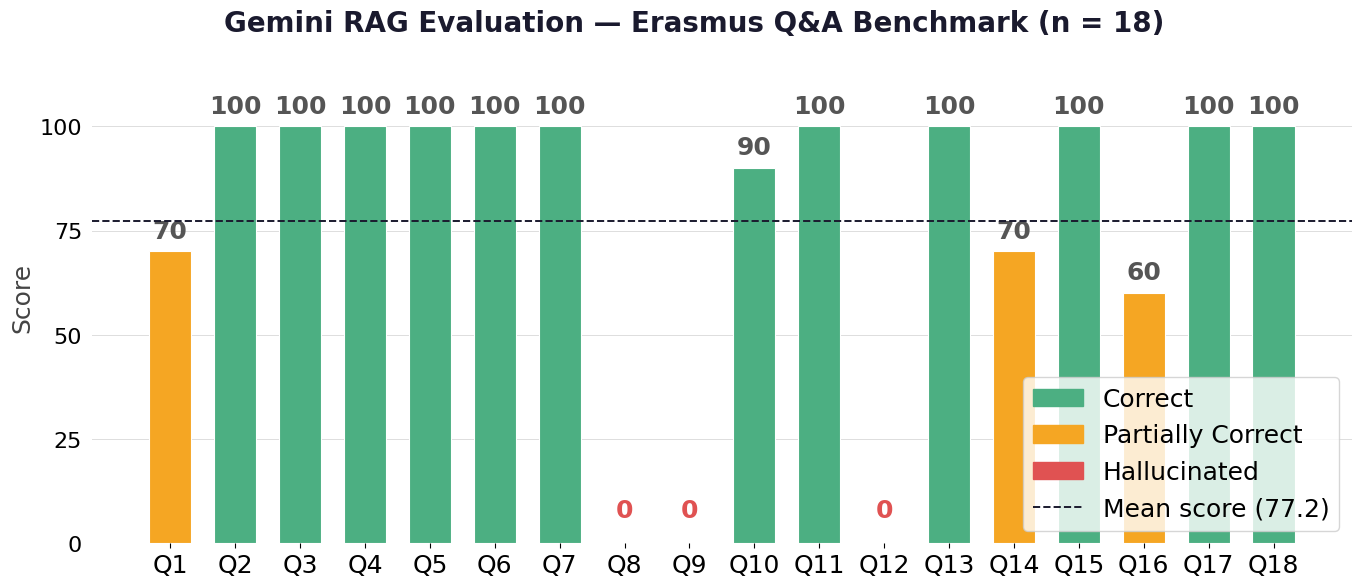
\includegraphics[width=0.475\textwidth]{per_question_scores.png}
    \caption{Per question scores evaluated with the Gemini API}
    \label{fig:scores}
\end{figure}

\subsection*{Categorical Breakdown}

The categorical assessment reveals a clearer picture of where the system succeeds and where it fails. Of the 18 questions:

\begin{itemize}
    \item \textbf{12 (66.7\%)} were rated \textsc{correct}, with an average score of 99.2, indicating that the system accurately retrieved and synthesised the relevant information in almost all such cases.
    \item \textbf{3 (16.7\%)} were rated \textsc{partially\_correct}, with an average score of 66.7. These responses captured some relevant information but omitted key details required for a complete answer.
    \item \textbf{3 (16.7\%)} were rated \textsc{hallucinated}, each receiving a score of 0. In all three cases the model incorrectly claimed it did not possess the requested information, directing the user to external sources, despite the answer being present in the knowledge base.
\end{itemize}

\subsection*{Analysis of Errors}

\paragraph{Hallucinated Responses.}
The three hallucinated responses (Q8, Q9, Q12) share a common failure mode: the model responded with a disclaimer stating it lacked the information, rather than retrieving it from the knowledge base. Concretely, Q8 asked how the Erasmus scholarship is paid (the correct answer being that 80\% is disbursed before the exchange and 20\% after completion), Q9 asked for the minimum and maximum duration of an exchange (2 and 12 months, respectively), and Q12 inquired whether language testing is mandatory before Erasmus (it is not, though some partner universities may require certificates). In all three instances the information was available in the indexed documents, suggesting that the retrieval step failed to surface the correct passage rather than the generation step fabricating an incorrect answer. This type of failure---where the model opts out rather than producing a plausible but wrong response---is conservative in one sense, but remains undesirable in a deployed assistant context.

\paragraph{Partially Correct Responses.}
The three partially correct responses (Q1, Q14, Q16) reflect a different failure mode: incomplete information synthesis. For Q1, the model correctly stated that FRI nominates the student to the partner university but omitted the subsequent step of applying directly to the host institution. For Q14, it correctly identified content similarity as a factor in course recognition upon return, but missed the additional condition that the outcome also depends on whether specific FRI programme requirements are met. For Q16, the model mentioned the FRI Erasmus office as a point of contact for problems encountered abroad, but failed to list other important support channels such as the host university coordinator, Erasmus mentor, the UL central office, or student tutors. These partial answers suggest that while retrieval is succeeding, the generation step is not consistently consolidating all relevant spans from the retrieved context.


%------------------------------------------------



\section*{Discussion}

The overall accuracy of the system is encouraging: two-thirds of all questions were answered correctly and completely, and the mean score exceeded 77 out of 100. However, the hallucination and partial correctness rates---each affecting approximately one in six questions---represent clear areas for improvement. The hallucination failures in particular suggest that the retrieval pipeline may be sensitive to the phrasing of certain queries, especially those involving procedural or numerical details that may be distributed across different parts of the source documents. Future work should explore query reformulation strategies, improved document chunking, and retrieval confidence thresholds to reduce the rate of uninformative opt-out responses. Addressing the partial completeness failures may additionally benefit from multi-passage fusion techniques or more explicit prompting of the generative model to enumerate all relevant details before producing a final answer.

%----------------------------------------------------------------------------------------
%   REFERENCE LIST
%----------------------------------------------------------------------------------------
\bibliographystyle{unsrt}
\bibliography{report}

\end{document}
